\section{Metodologías Empleadas \tutor{A lo largo de la memoria, abusas del uso de las mayúsculas. Salvo para inicios de frases o nombres propios, no es recomendable.}}
\tutor{El orden de las subsecciones es importante. Primero hay que hablar de las tecnologías, luego de las herramientas y por último de la metodología.}
En el desarrollo de Enterprise Event Solutions, se ha adoptado una metodología ágil basada en Scrum para asegurar que el proceso de creación 
fuera eficiente, organizado y adaptable a cambios y mejoras constantes. Aunque he trabajado solo en este proyecto, se ha implementado de manera 
rigurosa los principios de Scrum, enfocanose en alcanzar pequeños objetivos semanales y manteniendo una estructura organizada.

Cada semana, se han establecido objetivos específicos y alcanzables, lo que ha permitido avanzar de manera constante y mantener un alto nivel 
de motivación. Esta división en pequeños objetivos semanales ha ayudado a gestionar mejor el tiempo y a priorizar tareas, asegurando que cada 
funcionalidad de la aplicación se desarrolle de manera coherente y sin omisiones.

Para organizar y seguir el progreso, se ha utilizado un tablero de Trello. Este tablero ha sido una herramienta invaluable para no olvidar ideas o 
tareas pendientes. Cada tarjeta en el tablero representaba una tarea o idea específica, y he seguido un flujo de trabajo que incluía las siguientes 
etapas: por hacer, en progreso, y completado. Esta visualización clara del trabajo pendiente y del progreso realizado me ha permitido mantenerme 
enfocado y productivo.

Además, al final de cada semana, he realizado una revisión de los objetivos alcanzados y he ajustado el plan para la semana siguiente. Esta práctica 
de retrospectiva semanal ha sido fundamental para identificar áreas de mejora, solucionar problemas y asegurar que el proyecto siga avanzando de acuerdo 
con los objetivos establecidos.

En resumen, la adopción de la metodología Scrum, con su enfoque en pequeños objetivos semanales y el uso de un tablero Trello para la gestión de 
tareas, ha sido clave para el desarrollo exitoso de Enterprise Event Solutions. A pesar de trabajar solo, esta estructura me ha permitido mantener 
un alto nivel de organización, adaptabilidad y eficiencia en todo el proceso de desarrollo.


\begin{figure}[h]
    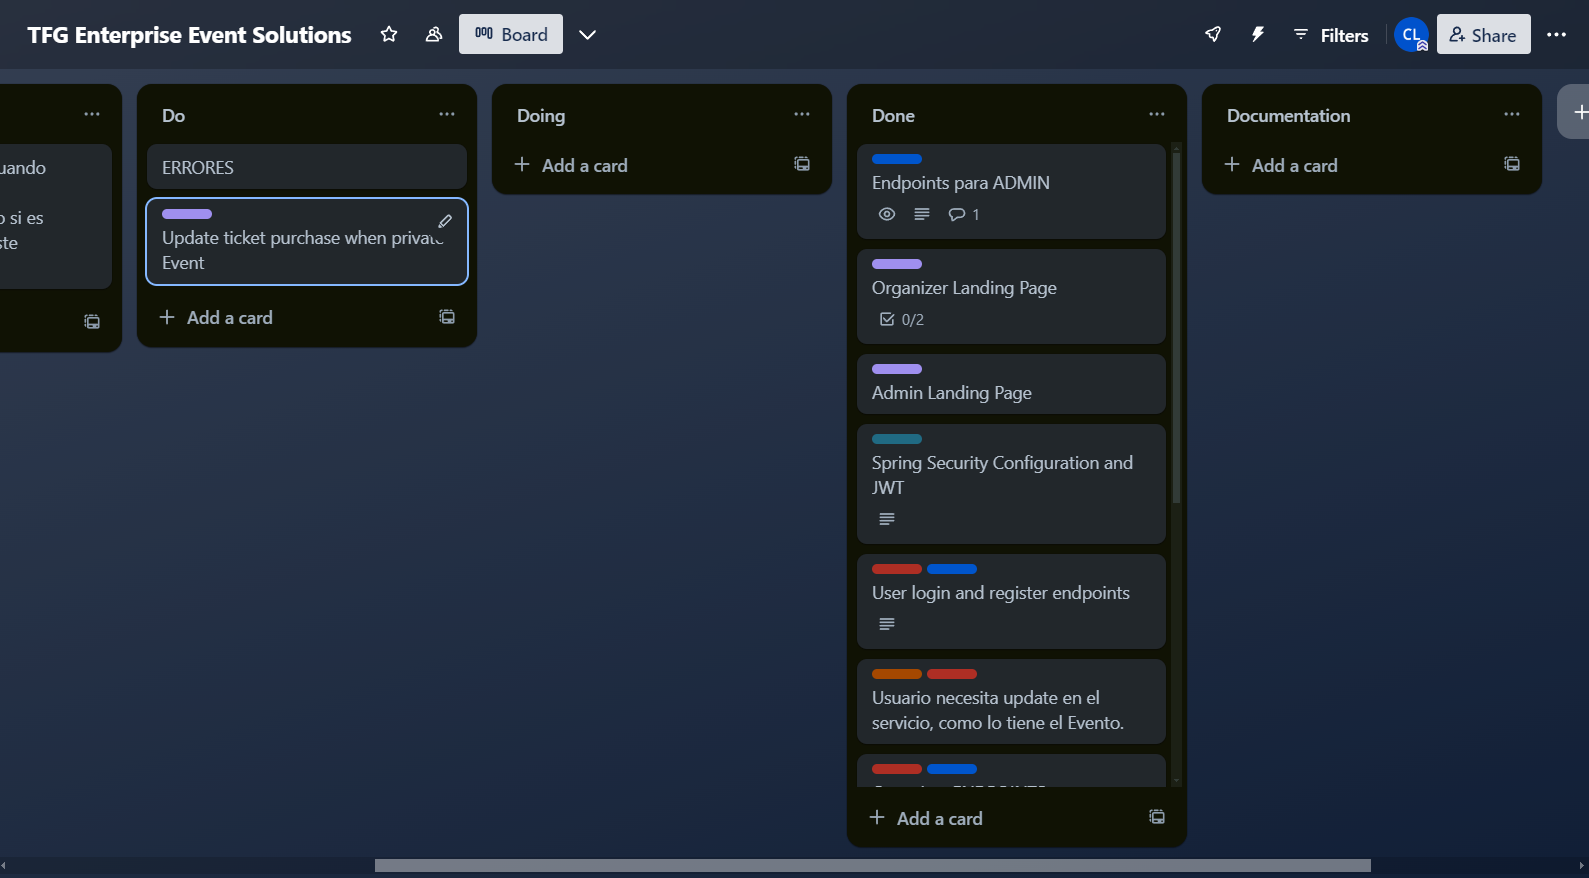
\includegraphics[width=\linewidth]{Trello.png}
    \caption{Trello en proceso.}
    \label{fig:metodologias1}
\end{figure}

En cuanto al desarrollo del código, se ha utilizado un flujo de trabajo basado en Pull Requests (PRs). Cada cambio o nueva 
funcionalidad se desarrollaba en una rama separada y se integraba al código principal solo después de ser revisada y aprobada 
mediante un Pull Request. Este enfoque ha permitido mantener un historial claro de los cambios, realizar revisiones detalladas y 
asegurar que cada nueva adición al código se integrara de manera ordenada y sin conflictos. Este método ha ayudado a mantener la disciplina y la organización en el
 desarrollo del software.

El uso de Pull Requests ha ofrecido múltiples ventajas en el proceso de desarrollo. En primer lugar, ha facilitado la identificación y 
resolución de errores antes de que los cambios se integren en la rama principal. Cada PR actuaba como un punto de control donde podía revisar 
el código, realizar pruebas y verificar la funcionalidad, asegurando que solo los cambios bien testeados y verificados fueran añadidos al proyecto.

Además, este método ha proporcionado una documentación implícita del desarrollo. Cada Pull Request incluía una descripción detallada de los 
cambios realizados, los problemas que solucionaba o las nuevas características añadidas. Esto no solo facilitó la gestión del proyecto, sino 
que también creó un registro histórico útil para futuras referencias y para cualquier otra persona que pueda colaborar en el futuro.

Trabajar con ramas separadas para cada nueva funcionalidad o cambio también ha sido crucial para mantener la estabilidad del proyecto. Al aislar el 
desarrollo de nuevas características en ramas dedicadas, he evitado que los cambios en progreso afecten la estabilidad de la rama principal. Esto ha 
sido especialmente útil para realizar experimentos o implementar grandes cambios sin riesgo de romper la aplicación.

Finalmente, la disciplina de utilizar Pull Requests, incluso trabajando solo, ha fomentado un enfoque metódico y estructurado al desarrollo. Este 
flujo de trabajo me ha obligado a pensar críticamente sobre cada cambio, a documentarlo adecuadamente y a asegurarse de que cada PR cumpliera con los 
estándares de calidad antes de ser fusionado. De hecho, para asegurar que todo cambio que se realizara estuviera controlado por si fuera necesario volver a versiones anteriores
hasta los cambios más pequeños se realizaban mediante PRs. Gracias a esto he consegido revertir cambios en momentos críticos del desarrollo.

\begin{figure}[h]
    \centering
    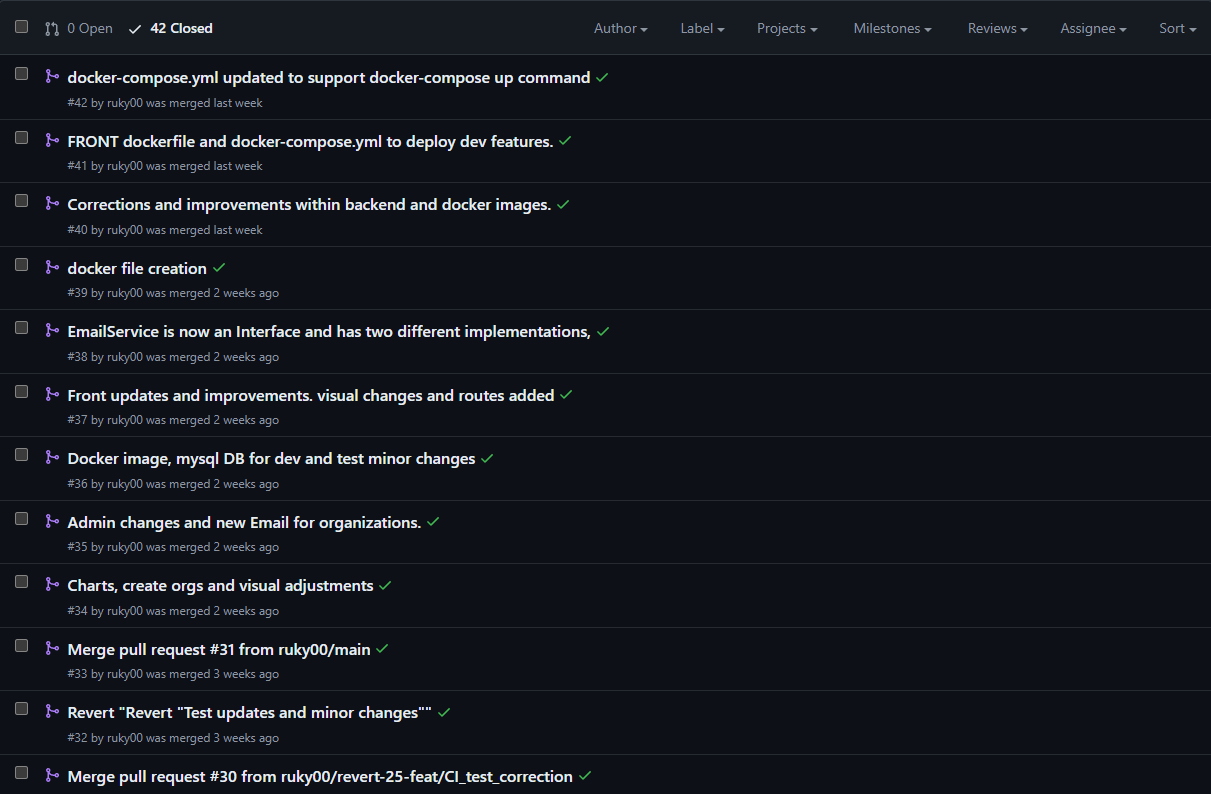
\includegraphics[width=\linewidth]{PRs.png}
    \caption{PRs del Repositorio.}
    \label{fig:metodologias2}
\end{figure}

En resumen, la adopción de la metodología Scrum, con su enfoque en pequeños objetivos semanales y el uso de un tablero Trello para la gestión de tareas, 
junto con el uso de Pull Requests, ha sido clave para el desarrollo exitoso de Enterprise Event Solutions.

El total desarrollo se ha realizado en un repositorio de GitHub donde se ha incluido un Readme.md utíl para el tanto el despliegue en producción como en desarrollo. De esta forma
aún sin la totalidad de los requerimientos, ya sea una cuenta de AWS o de Gmail, se podría hacer uso de la aplicación de forma local.  \textbf{\href{https://github.com/ruky00/EnterpriseEventSolutions}{Enlace al Repositorio}}



\section{Tecnologías Empleadas}

\subsection{SpringBoot}
Spring Boot\cite{spring-boot} es un framework Java que simplifica el desarrollo de aplicaciones web al eliminar la 
complejidad de la configuración manual. Ofrece configuración automática, empaquetado de aplicaciones independientes y un inicio rápido integrado, 
lo que permite a los desarrolladores crear aplicaciones de manera más rápida y eficiente, centrándose en la lógica de negocio en lugar de la configuración. 
Genial para el desarrollo de aplicaciones \textit{CRUD}\footnote{\textit{CRUD} es un acrónimo en inglés que se refiere a las operaciones 
básicas de manipulación de datos en aplicaciones informáticas: Create (Crear), Read (Leer), Update (Actualizar) y Delete (Eliminar).}.
\subsection{Maven}
Maven es una herramienta de gestión de proyectos Java que simplifica la estructuración, gestión de dependencias y automatización de la construcción. 
Permite definir dependencias en un archivo de configuración (pom.xml), ejecutar fases de construcción estandarizadas y gestionar repositorios 
centralizados de bibliotecas. Es ampliamente utilizado en el desarrollo Java por su integración con IDEs y su capacidad para proyectos multiproyecto, es decir,
permite la gestión de múltiples proyectos en un solo repositorio, lo que facilita la colaboración entre desarrolladores y la gestión.
\subsection{Vue.js}
Vue.js\cite{vue} es un popular marco de trabajo de código abierto para construir interfaces de usuario interactivas en aplicaciones web de una sola página. 
Se destaca por su enfoque centrado en el componente, su sintaxis declarativa y su eficiente sistema de reactividad. Vue.js facilita la construcción 
de aplicaciones web complejas al fomentar la reutilización de componentes y ofrecer herramientas integradas para la manipulación del DOM y la gestión 
del estado de la aplicación.

\subsection{MySQL}
MySQL es un sistema de gestión de bases de datos relacional de código abierto ampliamente utilizado en el desarrollo de 
aplicaciones web y empresariales. Destaca por su escalabilidad, rendimiento, fiabilidad y facilidad de uso. Ofrece opciones 
sólidas de seguridad y es compatible con una variedad de plataformas y lenguajes de programación. MySQL es una herramienta poderosa 
para gestionar eficientemente grandes volúmenes de datos y garantizar la integridad y disponibilidad de la información.

\subsection{IntelliJ}
IntelliJ IDEA es un entorno de desarrollo integrado (IDE) altamente productivo desarrollado por JetBrains. 
Diseñado para diversas tecnologías, ofrece una interfaz de usuario intuitiva y funciones avanzadas que mejoran la 
productividad del desarrollador. Con soporte para múltiples lenguajes y marcos de trabajo, integración con herramientas de desarrollo y 
características colaborativas, IntelliJ IDEA es una opción popular para el desarrollo de software en Java y otros lenguajes.

\subsection{VSCode}
Visual Studio Code (VSCode) es un IDE popular desarrollado por Microsoft, conocido por su versatilidad, rendimiento y comunidad activa.
 Ofrece características avanzadas y extensiones para diferentes lenguajes de programación. Es altamente personalizable y cuenta con una 
 amplia documentación disponible en su sitio web oficial.

\subsection{AWS S3}
AWS S3 es un servicio de almacenamiento en la nube ofrecido por Amazon Web Services. Destaca por su escalabilidad, durabilidad, seguridad y 
facilidad de uso. Permite almacenar grandes cantidades de datos de forma segura y acceder a ellos de manera eficiente a través de una interfaz 
intuitiva y una API robusta. Con una estructura de precios flexible, AWS S3 es una opción atractiva para empresas que buscan una solución de 
almacenamiento en la nube rentable y confiable.

\subsection{AWS EC2}
AWS EC2 es un servicio de cómputo en la nube proporcionado por Amazon Web Services. Destaca por su escalabilidad, flexibilidad y seguridad. 
Permite a los usuarios alquilar capacidad informática según sus necesidades, con opciones de pago por uso. Es fácil de usar y ofrece una variedad 
de opciones de implementación. En resumen, EC2 es una solución eficiente y confiable para ejecutar aplicaciones y cargas de trabajo en la nube.

\subsection{Docker}
Docker\cite{Docker} es una plataforma de código abierto que permite crear, implementar y ejecutar aplicaciones en contenedores. Destaca por su portabilidad, 
eficiencia y facilidad de uso. Con la tecnología de contenedores, Docker ofrece aislamiento de aplicaciones y escalabilidad, lo que simplifica el 
desarrollo y la administración de aplicaciones en diferentes entornos. En resumen, Docker es una herramienta fundamental para la creación y gestión 
eficiente de aplicaciones modernas.


\section{Resumen de las tecnologias}
La Tabla \ref{tabla:tecnologias_usos} recoge un resumen de las tecnologías empleadas para el desarrollo de Enterprise Event Solutions:

\tutor{Revisa la ortografía de la tabla (tecnología, creación, imágenes ...). Busca un corrector de ortografía en VSCode como ``Code Spell Checker''}
\begin{table}[h]
\begin{tabular}{ p{3cm} l  }

    \hline
    Tecnologia& Uso \\
    \hline
    SpringBoot   & Framework \\
    Maven &   Framework \\
    Vue.js & Framework  \\
    MySQL    & Tecnologia de BD \\
    IntelliJ&   Entorno de Desarrollo  \\
    VSCode& Entorno de Desarrollo \\
    AWS S3& Tecnologia de de BD en la nube  \\
    AWS EC2& Servidor web en la nube  \\
    Docker& Crecion de imagenes comprimidas para despliegue  \\
    \hline
   \end{tabular}
   \caption{Tecnologías y sus usos correspondientes}
   \label{tabla:tecnologias_usos}
\end{table}